\part{Einleitung}
In diesem Versuch soll die Funktionsweise eines Operationsverstärkers
veranschaulicht werden. Hierbei soll aber nicht der interne Aufbau und dessen 
Schaltbild veranschaulicht werden, sondern die externe Funktionsweise, wie 
dieser in der Praxis.

Operationen, die ein Operationsverstärker beispielsweise durchführen kann sind:
\begin{itemize}[noitemsep,nosep]
	\item Verstärkung
	\item Addition
	\item Integration
	\item Differentiation
\end{itemize}

\section{Theorie}
\cref{fig:Einleitung/SchaltbildOperationsverstärker} zeigt das Schaltsymbol, 
welches für einen beliebigen Operationsverstärker gilt. Dieser hat einen 
"`Plus"'-Eingang ($+$) und einen "`Minus"'-Eingang ($-$) und einen Ausgang A.

\begin{figure}[H]
	\centering
	\begin{subfigure}[t]{0.3\linewidth}
		\centering
		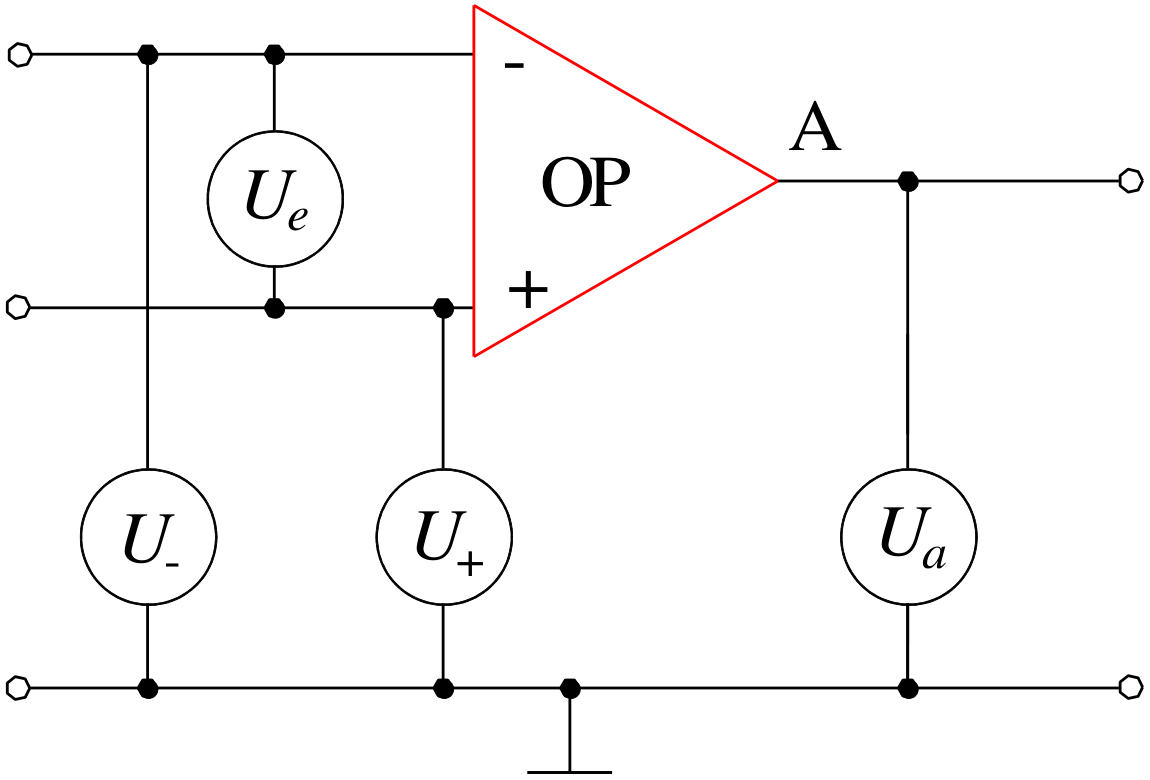
\includegraphics[width=\linewidth]{einleitung/schaltbildOP}
		\caption{Schaltbild eines Operationsverstärkers ({\color{red} rot}), 
		entnommen aus \cite{script}}
		\label{fig:Einleitung/SchaltbildOperationsverstärker}
	\end{subfigure}
	\quad
	\begin{subfigure}[t]{0.2\linewidth}
		\centering
		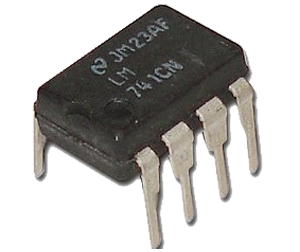
\includegraphics[width=\linewidth]{einleitung/741}
		\caption{Abbild eines Operationsverstärkers vom Typ 741, entnommen aus 
		\cite{image741}}
		\label{fig:Einleitung/Operationsverstärker}
	\end{subfigure}
	\quad
	\begin{subfigure}[t]{0.3\linewidth}
		\centering
		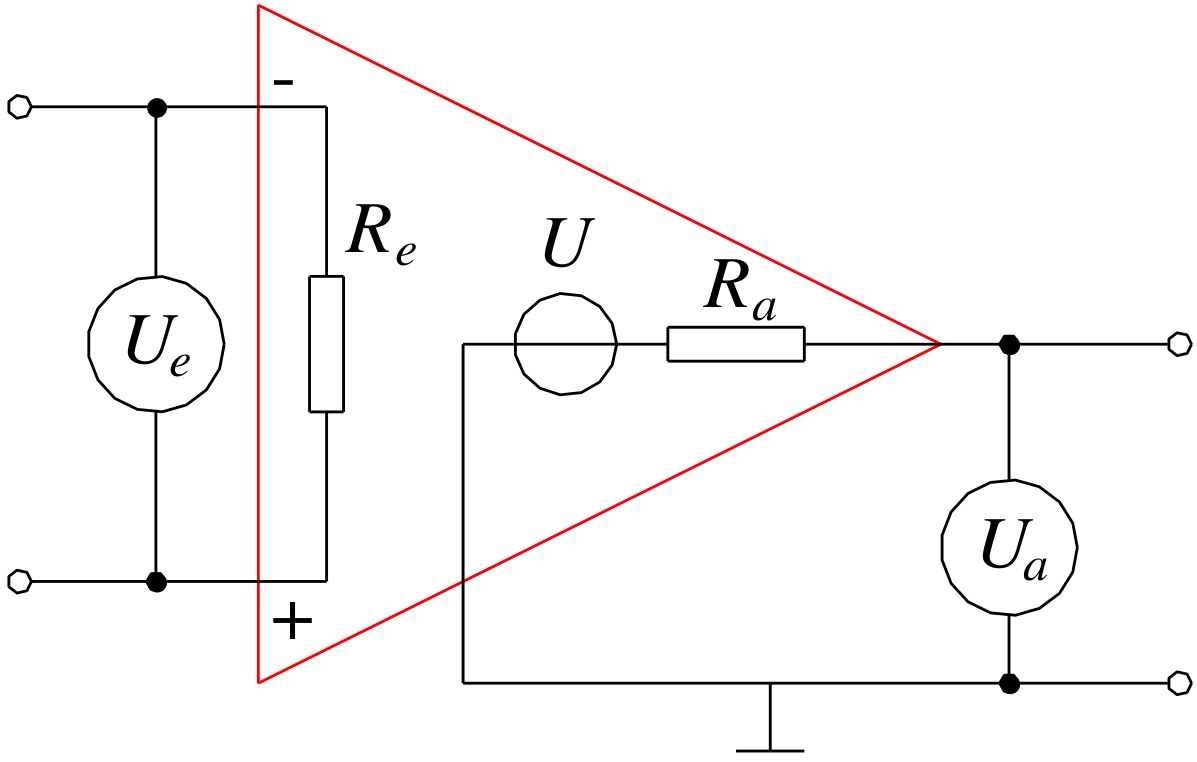
\includegraphics[width=\linewidth]{einleitung/ersatzSchaltbildOP}
		\caption{Ersatzschaltbild eines Operationsverstärkers ({\color{red} 
		rot}) zur Definition es Eingangswiderstandes $R_e$ und des 
		Ausgangswiderstandes $R_a$, entnommen aus \cite{script}}
		\label{fig:Einleitung/ErsatzschaltbildOperationsverstärker}
	\end{subfigure}
\end{figure}

Der Operationsverstärker verstärkt hierbei die 
\textsl{Eingangsspannungsdifferenz} $U_e$:
\begin{equation}\label{eq:Eingangsspannungsdifferenz}
	U_e = U_+ - U_-
\end{equation}
mit dem \textsl{Leerlaufverstärkungsfaktor} $V_0 > 0$, womit für die 
\textsl{Ausgangsspannung} $U_a$ gilt:
\begin{equation}\label{eq:Ausgangsspannung}
	U_a = V_0 \cdot U_e = V_0 \cdot \left(U_e = U_+ - U_-\right).
\end{equation}
Wenn $U_- = \qty{0}{\V}$ folgt aus \cref{eq:Ausgangsspannung}:
\begin{equation}
	U_- = \qty{0}{\V} \quad \rightarrow \quad U_a = V_0 \cdot U_+
\end{equation}
In diesem Fall haben sowohl die Eingangs- als auch die Ausgangsspannung das 
gleiche Vorzeichen. Daher wird der "`Plus"'-Eingang als 
\textsl{nicht-invertierender} Eingang bezeichnet. Im Gegensatz dazu gilt für 
den Fall
\begin{equation}
	U_+ = \qty{0}{\V} \quad \rightarrow \quad U_a = -V_0 \cdot U_-
\end{equation}
dass die Eingangsspannung $U_-$ und die Ausgangsspannung $U_a$ entgegengesetzte 
Vorzeichen haben. Daher wird der "`Minus"'-Eingang eines Operationsverstärkers 
auch \textsl{invertierender} Eingang genannt.

Ein idealer Operationsverstärker hat einen unendlich großen 
Leerlaufverstärkungsfaktor $V_0 \rightarrow \infty$ (vgl. 
\cref{fig:Einleitung/ErsatzschaltbildOperationsverstärker}), einen unendlich 
großen 
Eingangswiderstand $R_e \rightarrow \infty$ (vgl. 
\cref{fig:Einleitung/ErsatzschaltbildOperationsverstärker}), einen 
verschwindend kleinen Ausgangswiderstand $R_a \rightarrow 0$ (vgl. 
\cref{fig:Einleitung/ErsatzschaltbildOperationsverstärker}) und eine 
frequenzunabhängige Verstärkung. Ein realer Operationsverstärker weicht 
natürlich von diesem Idealvorstellungen ab: die Widerstände sind weder 
unendlich groß noch verschwindend klein, auch der Leerlaufverstärkungsfaktor 
hat seine Grenze und die Verstärkung findet frequenzabhängig statt.

Für die folgenden Überlegungen wird jedoch trotzdem der Operationsverstärker 
als eine "`Black Box"' angenommen und mit den idealen Eigenschaften betrachtet.
